\documentclass[11pt,a4paper,onside,UTF8]{article}
\usepackage{geometry}
	\geometry{left=2cm,right=2cm,top=2.5cm,bottom=3cm}
\usepackage[utf8]{inputenc}
\usepackage[english]{babel}
\usepackage{lipsum}
\usepackage{bm}
\usepackage{upgreek}

\usepackage{amsmath}
% mathtools for: Aboxed (put box on last equation in align envirenment)
\usepackage{microtype} %improves the spacing between words and letters

\usepackage{xeCJK,paralist,enumerate,booktabs,multirow,graphicx,float,setspace}
	\setlength{\parindent}{2em}%正文首行缩进两个汉字
% \usepackage{ctex}
%     \setmainfont{Times New Roman}

%% COLOR DEFINITIONS

\usepackage[svgnames]{xcolor} % Enabling mixing colors and color's call by 'svgnames'

\definecolor{MyColor1}{rgb}{0.2,0.4,0.6} %mix personal color
\newcommand{\textb}{\color{Black} \usefont{OT1}{lmss}{m}{n}}
\newcommand{\blue}{\color{MyColor1} \usefont{OT1}{lmss}{m}{n}}
\newcommand{\blueb}{\color{MyColor1} \usefont{OT1}{lmss}{b}{n}}
\newcommand{\red}{\color{LightCoral} \usefont{OT1}{lmss}{m}{n}}
\newcommand{\green}{\color{Turquoise} \usefont{OT1}{lmss}{m}{n}}

\DeclareMathOperator{\trace}{trace}
\DeclareMathOperator{\diag}{diag}

%% FONTS AND COLORS

%    SECTIONS

\usepackage{titlesec}
	\newfontfamily\sectionef{Times New Roman}
	\setCJKfamilyfont{FZHeiTi}{黑体}
	\newcommand{\sectioncf}{\CJKfamily{FZHeiTi}}
	\titleformat*{\section}{\large\bfseries\sectioncf\sectionef}
	\titleformat*{\subsection}{\normalsize\bfseries\sectioncf\sectionef}
\usepackage{sectsty}
%%%%%%%%%%%%%%%%%%%%%%%%
%set section/subsections HEADINGS font and color
\sectionfont{\color{MyColor1} \usefont{OT1}{lmss}{b}{n}}  % sets colour of sections
\subsectionfont{\color{MyColor1}\usefont{OT1}{lmss}{b}{n}}  % sets colour of sections

%set section enumerator to arabic number (see footnotes markings alternatives)
\renewcommand\thesection{\arabic{section}.} %define sections numbering
\renewcommand\thesubsection{\thesection\arabic{subsection}} %subsec.num.

%define new section style
\newcommand{\mysection}{
\titleformat{\section} [runin] {\usefont{OT1}{lmss}{b}{n}\color{MyColor1}} 
{\thesection} {3pt} {} } 


%	CAPTIONS
\usepackage{caption}
\usepackage{subcaption}
%%%%%%%%%%%%%%%%%%%%%%%%
% \captionsetup[figure]{labelfont={color=Turquoise}}


%		!!!EQUATION (ARRAY) --> USING ALIGN INSTEAD
%using amsmath package to redefine eq. numeration (1.1, 1.2, ...) 
\renewcommand{\theequation}{\thesection\arabic{equation}}



\makeatletter
\let\reftagform@=\tagform@
\def\tagform@#1{\maketag@@@{(\ignorespaces\textcolor{red}{#1}\unskip\@@italiccorr)}}
\renewcommand{\eqref}[1]{\textup{\reftagform@{\ref{#1}}}}
\makeatother
\usepackage[colorlinks,linkcolor=blue,urlcolor=blue]{hyperref}%超链接

% For labeling top of page on every page but first one:
\usepackage{fancyhdr}

% PREPARE TITLE:
\title{\blue Medical Statistics \\
\blueb Homework 1}
\author{Class 3 ~~ 莫润冰 ~~ 20980131}
\date{}

\renewcommand{\rmdefault}{phv} % Arial Font
\renewcommand{\sfdefault}{phv} % Arial Font
\usepackage{datetime}

\pagestyle{fancy}
\fancyhead{}
% \fancyhead[CO,CE]{{\small{{\bf{Homework Number}} - Class Name - Semester - Your Name}}}
\fancyhead[L]{Medical Statistics}
\fancyhead[R]{\shortmonthname[\the\month], \the\year}
\fancyhead[C]{
\normalsize{HW1}
}

\usepackage{listings}
\usepackage{color}

\definecolor{dkgreen}{rgb}{0,0.6,0}
\definecolor{gray}{rgb}{0.5,0.5,0.5}
\definecolor{mauve}{rgb}{0.58,0,0.82}

\lstset{ %
	language=R,                % the language of the code
	basicstyle={\footnotesize\usefont{OT1}{lmss}{m}{n}},           % the size of the fonts that are used for the code
	numbers=left,                   % where to put the line-numbers
	numberstyle=\tiny\color{gray},  % the style that is used for the line-numbers
	stepnumber=1,                   % the step between two line-numbers. If it's 1, each line 
									% will be numbered
	numbersep=5pt,                  % how far the line-numbers are from the code
	backgroundcolor=\color{white},      % choose the background color. You must add \usepackage{color}
	showspaces=false,               % show spaces adding particular underscores
	showstringspaces=false,         % underline spaces within strings
	showtabs=false,                 % show tabs within strings adding particular underscores
	frame=single,                   % adds a frame around the code
	rulecolor=\color{black},        % if not set, the frame-color may be changed on line-breaks within not-black text (e.g. commens (green here))
	tabsize=2,                      % sets default tabsize to 2 spaces
	captionpos=b,                   % sets the caption-position to bottom
	breaklines=true,                % sets automatic line breaking
	breakatwhitespace=false,        % sets if automatic breaks should only happen at whitespace
	title=\lstname,                   % show the filename of files included with \lstinputlisting;
									% also try caption instead of title
	keywordstyle=\color{red},          % keyword style
	commentstyle=\color[cmyk]{1,0,1,0},       % comment style
	stringstyle=\color{MyColor1},         % string literal style
	escapeinside={\%*}{*)},            % if you want to add LaTeX within your code
	morekeywords={*,...}               % if you want to add more keywords to the set
}



%%%%%%%%%%%%%%%%%%%%%%%%%%%%%%%%%%%%%%%%%%%%%%%%%%%%%%%%%%%%%%%%%%%%%%%%%%%%%%%%%%%%%%%
%%%%%%%%%%%%%%%%%%%%%%%%%%%%%%%%%%%%%%%%%%%%%%%%%%%%%%%%%%%%%%%%%%%%%%%%%%%%%%%%%%%%%%%
\begin{document}
\maketitle

\renewcommand{\thefootnote}{\fnsymbol{footnote}}
\footnotetext[1]{Github repo: \url{https://github.com/MoRunbing/Medical_Statistics }}
\footnotetext[2]{E-mail: \url{morb@mail2.sysu.edu.cn}}

\section{Exercise 1}

\begin{figure}[H]
	\centering
	\subfloat[]{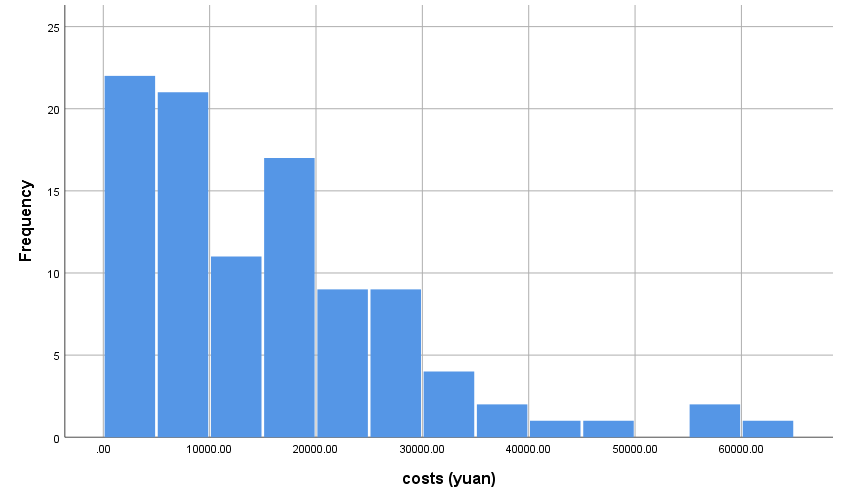
\includegraphics[width=0.5\textwidth]{fig//histogram.png}}
	\subfloat[]{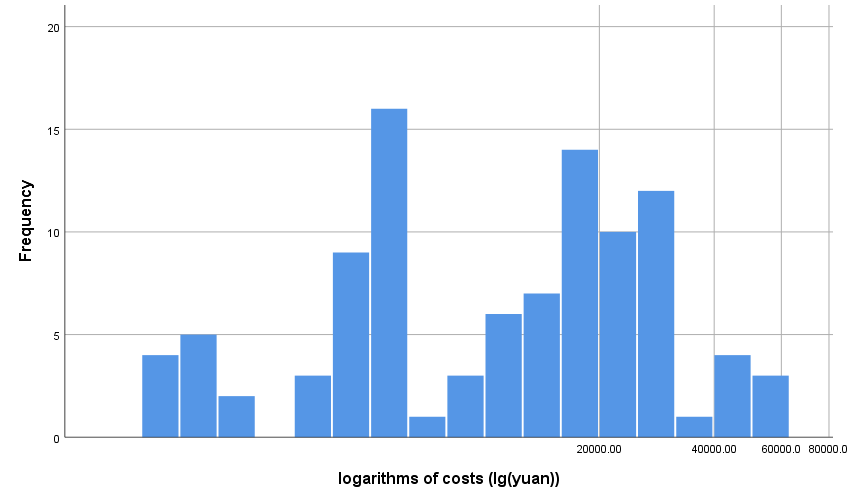
\includegraphics[width=0.5\textwidth]{fig//histogram_log.png}}
	\caption{Histogram of total treatment and rehabilitation costs in thousands}
\end{figure}
The histogram is higher around the center and shorter on two sides but not symmetric.
The tail on the positive side is much longer than the negative side, and it is called positive skew. 
This represents that the majority of people's expenses in treatment and rehabilitation are below average.

\subsection{Measurement of Average}
As the histogram of cost is positive skew, and the logrithms is close to symmetric, the geometric mean may better represent the average level of total treatment and rehabilitation costs than the arithmetic mean.

\begin{equation}
	arithmetic \ mean: \bar{x} = \frac{1}{n}\sum_{i = 1}^{n} x_i = 15550.30
\end{equation}
\begin{equation}
	geometric \ mean: \bar{x}= \sqrt[n]{x_1 x_2 \cdots x_n} = 10445.64
\end{equation}
\small{*total number of patients n = 100; $x_i$ represents the cost of $i^{th}$ patient}
\\ \hspace*{\fill} \\

Since the histogram is taller around the center and shorter on two sides, but not pocessses symmetric feature. 
Median can also present the average level well. 
\\ \hspace*{\fill} \\

\begin{equation}
	median: M_d = 13092.50
\end{equation}

Median is smaller than the arithmetic mean, which further proves the positive skew of the histogram.

\subsection{Measurement of Variation}

\subsubsection*{Range:}
\begin{equation}
	maximum\ value = 60790.00
\end{equation}
\begin{equation}
	minimum\ value = 1435.00
\end{equation}
\begin{equation}
	range = maximum\ value - minimum\ value = 59355.00
\end{equation}

\subsubsection*{$Q_3-Q_1$:}

$Q_3$ is 75 percentile of patients' costs, which indicates the value with a rank most closely to $75\%$ of the patients, 
while $Q_1$ is 25 percentile.
$Q_3-Q_1$ discribes sample variance better than range since it excludes those extreme values.

\begin{equation}
	Q_3 = 21176.25
\end{equation}
\begin{equation}
	Q_1 = 5082.5
\end{equation}
\begin{equation}
	Q_3-Q_1 = 16093.75
\end{equation}

\subsubsection*{Varience and Standard Deviation:}
Varience and standard deviation show more individual information than those values calculated above.
\begin{equation}
	variance: S^2 = \frac{\sum_{i=1}^{n} \left(x_i-\bar{x}\right)^2}{n-1} = 172369611.53
\end{equation}
\begin{equation}
	standard\ deviation: S = \sqrt{S^2} = 13128.96 
\end{equation}

\subsubsection*{Coefficient of Variation:}
Coefficient of variation is a dimentionless value suitable for comparison between different datasets.

\begin{equation}
	coefficient\ of\ variation: CV = \frac{S}{\bar{x}} =  0.84
\end{equation}


\end{document}